% !TEX root = ../main.tex

\chapter{Oplossingen van het stelsel.}
\label{Oplossingen van het stelsel}

\section{Methode van Euler.}
De methode van Euler is numerieke methode voor het oplossen van differentiaalvergelijkingen met een beginwaarde. De methode gaat uit van de definitie van afgeleide: $f'(x) = \lim_{h\to0}\frac{f(x+h)-f(x)}{h}$. Door deze vergelijking om te schrijven krijgen we de volgende vergelijking $\lim_{h\to0}f(x+h) = f(x) + \lim_{h\to0}hf'(x)$. De methode van Euler benadert nu $f(x+h)$ door $h$ klein te kiezen en $f(x+h) = f(x) + hf'(x)$ te stellen.

Voor de differentiaalvergelijkingen van de bioreactor:
\begin{align*}
	\frac{\dd X}{\dd t} &= \alpha_1 \frac{S}{1 + S} X - X,\\
	\frac{\dd S}{\dd t} &= - \frac{S}{1 + S}X - S + \alpha_2,
\end{align*}
komt de oplossing er nu als volgt uit te zien:
\begin{align*}
	X(t+h) &= X(t) + h \left( \alpha_1 \frac{S(t)}{1 + S(t)} X(t) - X(t) \right),\\
	S(t+h) &= S(t) + h \left(- \frac{S(t)}{1 + S(t)}X(t) - S(t) + \alpha_2 \right).
\end{align*}

\section{Concentratie tegen tijd.}
Nu we een benadering van de oplossingen hebben kunnen we deze voor verschillende beginwaarden en verschillende waarden $\alpha_1$ en $\alpha_2$ uitzetten tegen de tijd.
\newpage
\begin{figure}[h]
    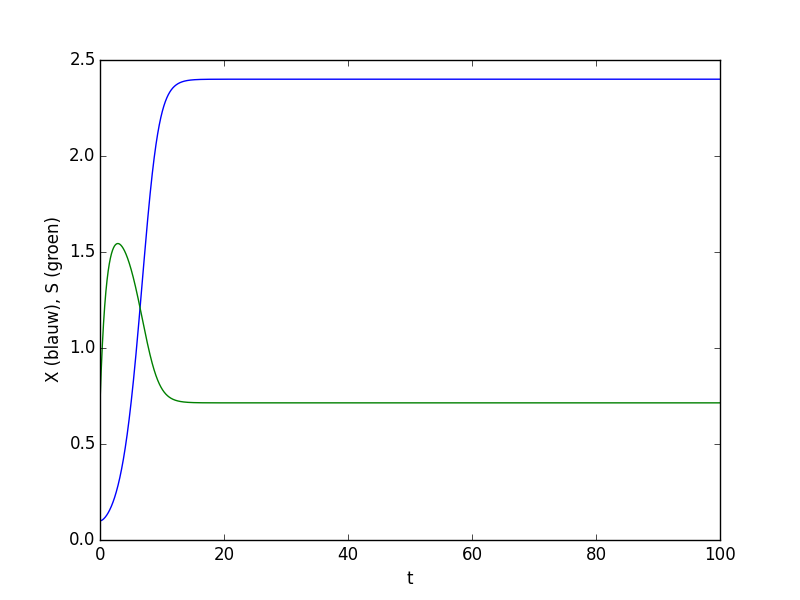
\includegraphics[width=0.5\textwidth]{../images/figure_1.png}
    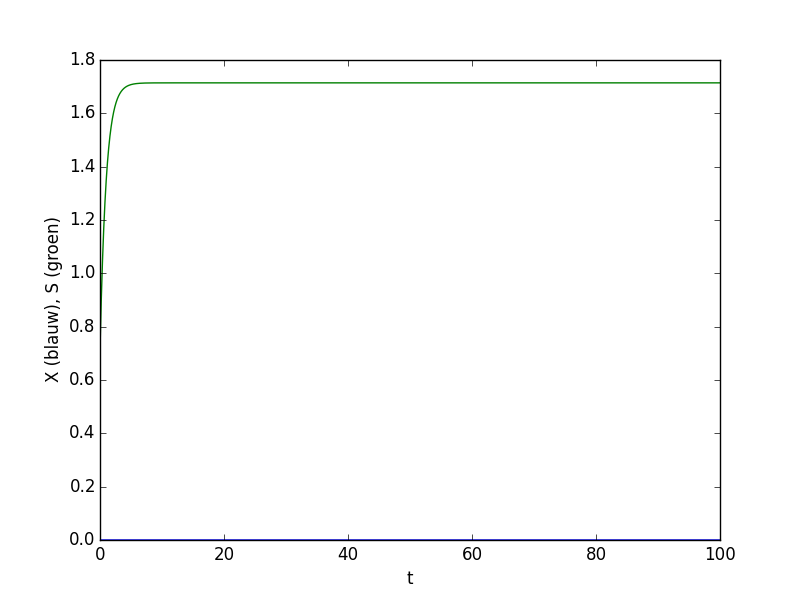
\includegraphics[width=0.5\textwidth]{../images/figure_2.png}
    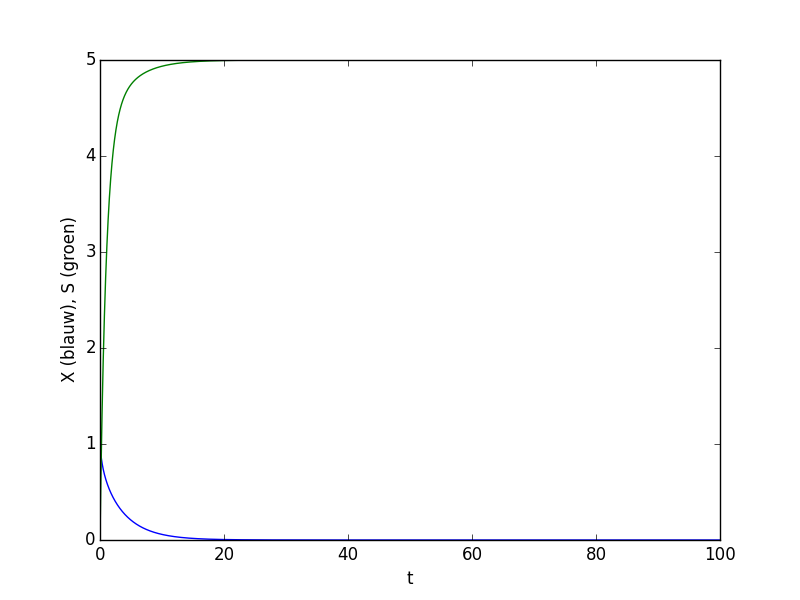
\includegraphics[width=0.5\textwidth]{../images/figure_3.png}
    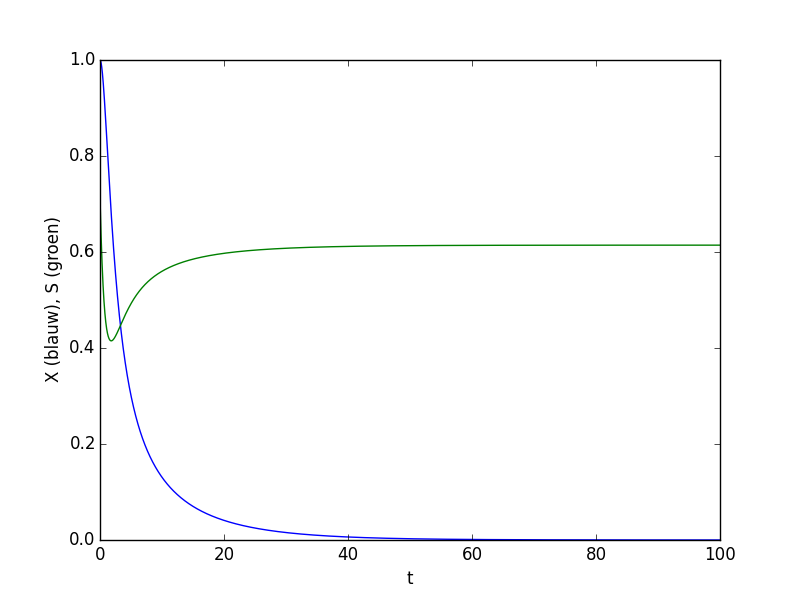
\includegraphics[width=0.5\textwidth]{../images/figure_4.png}
    \caption{Bacterie- en voedselconcentratie tegen de tijd.}
    \label{fig:tijd_plots}
\end{figure}

In de figuur linksboven is $\alpha_1 = 2.4 > 1$ en $\alpha_2 = \frac{1}{\alpha_1-1}+1>\frac{1}{\alpha_1-1}$. In dit geval is er een stabiel evenwicht waarbij er een positief aantal bacteri\"en in de reactor blijft.
Rechtsboven is de beginwaarde van de bacterieconcentratie 0. In dit geval gaat de voedselconcentratie naar een evenwicht toe en blijft de bacterieconcentratie 0.
Linksonder is $\alpha_1 = 0.9 < 1$. In dit geval gaat de bacterieconcentratie naar 0 toe. De reden hiervoor is te trage voortplanting.
Rechtsonder is $\alpha_1 = 2.4 > 1$, maar $\alpha_2 = \frac{1}{\alpha_1-1}-.1<\frac{1}{\alpha_1-1}$. In dit geval zien we weer dat de bacterieconcentratie naar 0 toe gaat. De reden hiervoor is voedseltekort.

We zien nu dus dat de voedsel- en bacterieconcentratie altijd naar een evenwicht convergeren.

\section{Het fasevlak.}

In een fasevlak kunnen we mooi zien waar dat evenwicht zich daadwerkelijk bevindt. We kijken weer naar de zelfde gevallen als in de grafieken in figuur 4.1.

De lichtblauwe lijn geeft hierin de het verloop van de voedsel- en bacterieconcentratie aan, op de donkerblauwe lijn is de bacterieconcentratie in evenwicht en op de groene lijn is de voedselconcentratie in evenwicht. Op het punt waar de donkerblauwe en de groene lijn elkaar kruisen staat een ster. Op dit punt is de hele bioreactor in evenwicht.

\begin{figure}[h]
    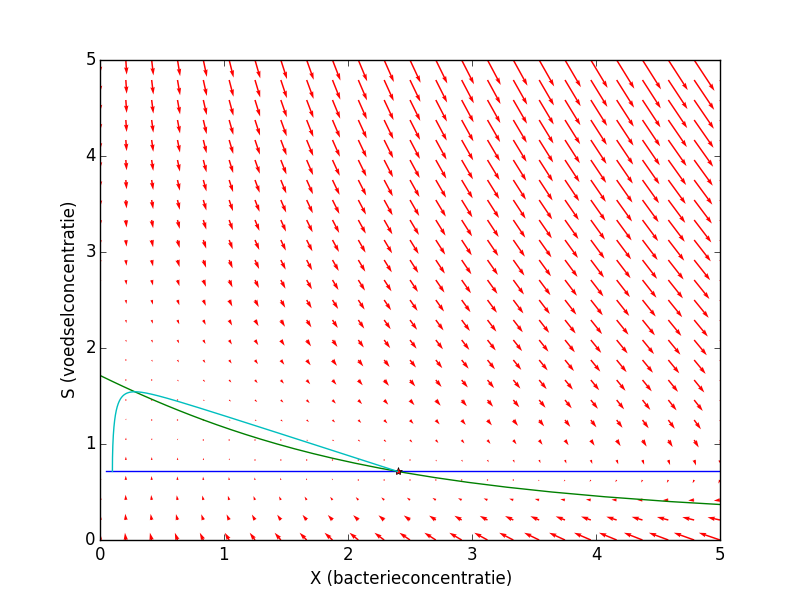
\includegraphics[width=0.5\textwidth]{../images/fase_1.png}
    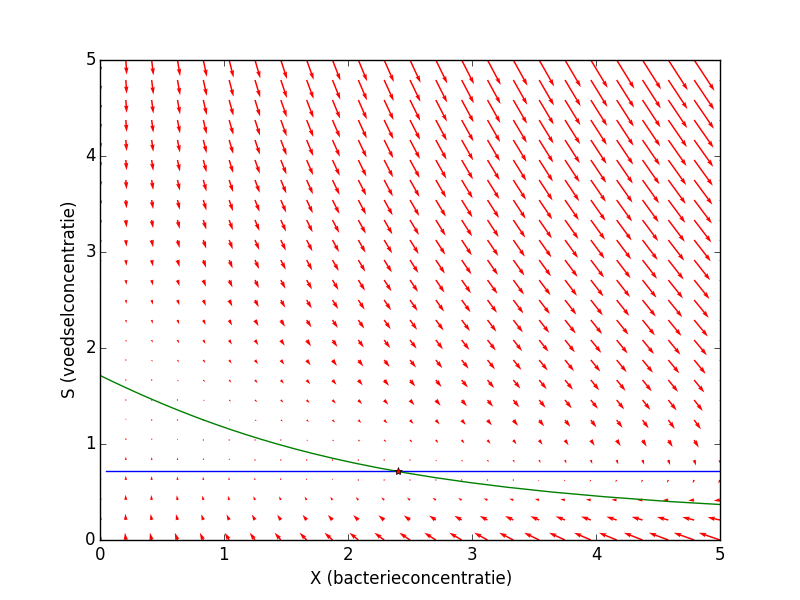
\includegraphics[width=0.5\textwidth]{../images/fase_2.png}
    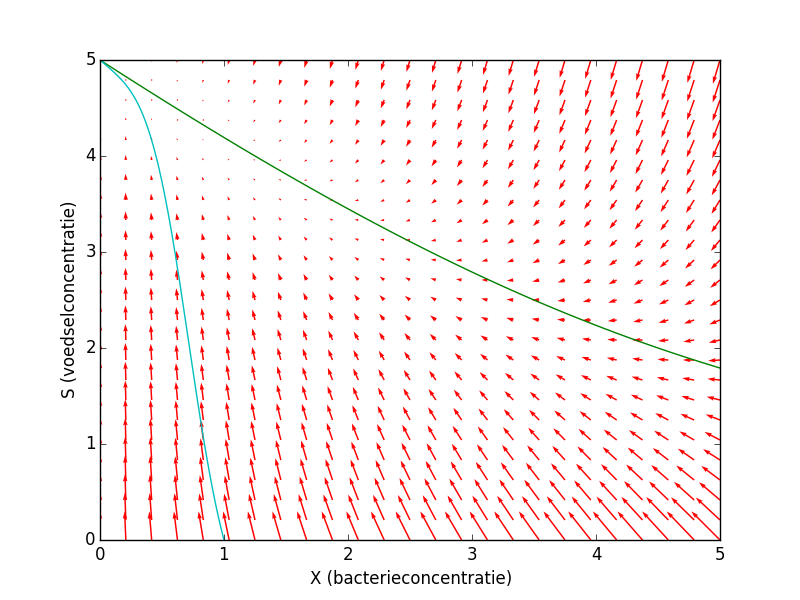
\includegraphics[width=0.5\textwidth]{../images/fase_3.png}
    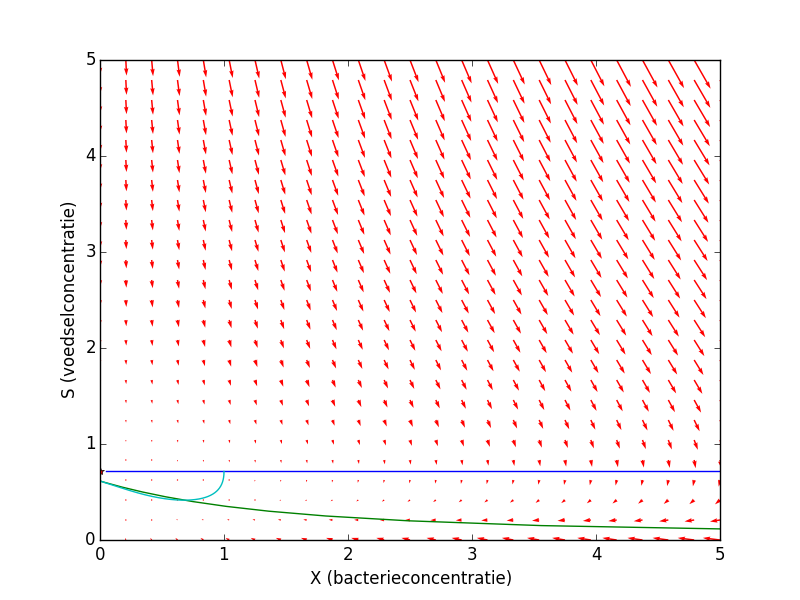
\includegraphics[width=0.5\textwidth]{../images/fase_4.png}
    \caption{Bacterie- en voedselconcentratie tegen elkaar.}
    \label{fig:fase_plots}
\end{figure}










